\documentclass[a4paper]{exam}

\usepackage{graphicx}

\usepackage{siunitx}
\DeclareSIUnit{\revolution}{rev}
\DeclareSIUnit{\rpm}{\revolution\per\minute}
\DeclareSIUnit{\lightyear}{ly}

\begin{document}
  \section*{L3 Physics: Questions for 1.1-1.5}
  Majority taken from Knight chap. 6, 7, 10, 11, 13.

  \paragraph{Remarks.} These questions range from easy (some maybe at Y12 level) to scholarship level. Some of them might require calculus to solve.
  I have not marked the difficulty level (they are not in order), nor have I indicated which require calculus. If you think a problem is too difficult,
  you should try to solve it until you get to the part which is too difficult or requires calculus; being able to set problems up like this is a very
  important skill.

  There are more problems here than you are expected to solve: the guideline I will give is that you should solve as many as you feel like you \emph{should}
  solve, and no less. Scholarship students, please attempt all the problems.

  \begin{questions}
    \question A \SI{20}{\gram} blob of clay travelling east at \SI{3.0}{\metre\per\second} collides with a \SI{30}{\gram} blob travelling
              north at \SI{2.0}{\metre\per\second}. What are the speed and direction of the combined blob? Give the direction as an angle
              north of east.
    \question Squids rely on jet propulsion to move about. A \SI{1.50}{\kilo\gram} squid (this mass includes the water within the squid) drifting
              at \SI{0.40}{\metre\per\second} suddenly ejects \SI{0.10}{\kilo\gram} of water to get itself moving at \SI{2.50}{\metre\per\second}
              in the same direction as it was drifting. If drag is ignored over the small period of time needed to expel the water, what is the
              water's ejection speed relative to the initial speed of the squid?
    \question A cannon tilted up at an angle of \ang{30} fires a cannon ball at \SI{75}{\metre\per\second} from the top of a \SI{12}{\metre} tall
              wall. What is the impact speed of the ball when it hits the ground?
    \question Blocks with masses 2, 3, and 5 (all in kilograms) are lined up in a row on a frictionless table. A force of \SI{10}{\newton}
              is applied to the \SI{2}{\kilo\gram} block to get all three moving. What is the force exerted by the \SI{3}{\kilo\gram} block (a) on
              the \SI{5}{\kilo\gram} block, (b) on the \SI{2}{\kilo\gram} block? [Hint: all three blocks will have the same... what?]
    \question An object moving along a surface experiences a friction force. The usual model for this is the force law $ F_\text{fric} = \mu N $,
              where $ \mu $ is a number called the \emph{coefficient of friction} that depends on the surface, and $ N $ is the normal force
              of the surface on the object being moved.
      \begin{parts}
        \part What are the units of $ \mu $?
        \part A \SI{4000}{\kilo\gram} truck is parked on a \ang{15} slope. How large is the friction force on the truck if the coefficient
              of friction between the tires and the road is 0.90?
        \part A bullet of mass $ m $ is fired into a block of mass $ M $ that is at rest. The block, with bullet embedded, slides a distance $ d $
              along a horizontal surface with coefficient of friction $ \mu $ before stopping. Show that the speed of the bullet at the point of
              impact is
              \begin{displaymath}
                v_\text{bullet} = \left(1 + \frac{M}{m}\right)\sqrt{2\mu g d}
              \end{displaymath}
              where $ g $ is the acceleration due to gravity.
      \end{parts}
    \question A bungee jumper, mass \SI{80}{\kilo\gram}, jumps off a bridge \SI{100}{\metre} above a river. For practical purposes we may model
              the bungee cord (length \SI{30}{\metre}) as a spring with spring constant \SI{40}{\newton\per\metre}. How far is the jumper above
              the water when the cord reaches its maximum elongation?
    \question A planet, mass $ m $, is orbiting a star, mass $ M $. The distance between their centres of mass is a constant $ R $, and the period
              of the orbit (that is, the time for one orbit to be completed) is $ T $. Show that
              \begin{displaymath}
                \frac{GM}{4\pi^2} T^2 = R^3.
              \end{displaymath}
              This is Kepler's third law of planetary motion.
    \question A \SI{200}{\gram} ball is dropped from a height of \SI{2.0}{\metre}, bounces on a hard floor, and rebounds to a height of \SI{1.5}{\metre}.
              The following figure shows the impulse received by the floor. What is the maximum force $ F_\text{max} $ exerted by the ball by the floor?

              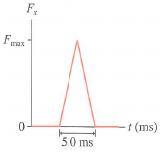
\includegraphics[width=0.2\textwidth]{impulse_curve}
    \question
      \begin{parts}
        \part Show that the gravitational potential energy associated with a system of two masses $ m $ and $ M $ with a distance $ r $ between
              their centres of mass is
              \begin{displaymath}
                U_g = -\frac{GMm}{r}.
              \end{displaymath}
              (Hint: this is exercise 1.23.1 in the notes.)
        \part A \SI{1000}{\kilo\gram} rocket is fired straight up from the surface of the earth. Assuming that the forces acting on the rocket
              due to the earth's rotation are negligible, with which speed does the rocket need to be fired for it to escape the gravitational
              pull of the earth and never return?
      \end{parts}
    \question Two Jupiter-sized (\SI{1.90e27}{\kilo\gram} mass, \SI{6.99e7}{\metre} radius) planets are released from rest \SI{1.0e11}{\metre} apart. What
              are their speeds when they crash into each other?
  \end{questions}

\vspace*{\fill}
This version: \today

\end{document}
